\usepackage{graphicx}

\lstset{
style=python,
morekeywords={[2]
}
}

\section{Wbudowane typy danych}\label{sec:data_types}
\begin{frame}{Typy danych}
    W Pythonie mamy 5 prostych typów danych:
    \begin{itemize}
        \item float() - reprezentuje liczby rzeczywiste \footnote{Nie jest to do końca prawda, o czym przekonasz się na kolejnych slajdach.} \\
        \item int() - reprezentuje liczby całkowite \\
        \item str() - reprezentuje napisy - łańcuchy znaków \\
        \item bool() - reprezentuje wartości logiczne \\
        \item complex() - reprezentuje liczby urojone \\
    \end{itemize}
    Oraz 4 typy złożone:
    \begin{itemize}
        \item list() - reprezentuje zmienną grupę danych \\
        \item tuple() - reprezentuje uporządkowaną strukturę danych \\
        \item dict() - reprezentuje grupę danych, które da się indeksować \\
        \item set() - reprezentuje zbiór danych w rozumieniu teorii zbiorów \\
    \end{itemize}
\end{frame}
\begin{frame}{Proste typy danych}
    \lstinputlisting{data_structures/code/basic_types_1.py}
\end{frame}
\begin{frame}{Proste obliczenia}
    \lstinputlisting{data_structures/code/basic_types_2.py}
\end{frame}
\begin{frame}{Struktura danych - lista}
    \begin{small}
        \begin{itemize}
            \item list() \\
            \item lista jednokierunkowa działa jak stos rezerwowy w grze pasjans - możemy
            podglądać jedną kartę i przesuwać się tylko do następnej \\
            \item lista dwukierunkowa pozwala przesuwać się w obie strony \\
            \item do listy możemy dodawać elementy w dowolne miejsce i usuwać je \\
            \item listy przyjaciół: [Ala, Ola, Ela] oraz [Ela, Ala, Ola] są równoważne - kolejność
            nie ma znaczenia \\
            \item jeśli powyższą listę potraktujemy jako posortowaną listę przyjaciół według jakiegoś
            kryterium, np. który z przyjaciół najlepiej gotuje, albo którą z przyjaciółek najchętniej
            zaproszę na studniówkę - wtedy kolejność będzie mieć znaczenie
        \end{itemize}
    \end{small}
    \begin{table}
        \centering
        \begin{tabular}{c|c|c|c|c|c|c}
            \cline{2-2} \cline{4-4} \cline{6-6}
            HEAD \longrightarrow & DATA & \multirow{ 2}{*}{\nearrow} & DATA & \multirow{ 2}{*}{\nearrow} & DATA & \\
            \cline{2-2} \cline{4-4} \cline{6-6}
            & NEXT & & NEXT & & NEXT & \longrightarrow NULL \\
            \cline{2-2} \cline{4-4} \cline{6-6}
        \end{tabular}
    \end{table}
\end{frame}
\begin{frame}{Struktura danych - krotka}
    \begin{itemize}
        \item tuple() \\
        \item para, trójka, czwórka, czyli ogólnie krotka \\
        \item uporządkowany rekord który ma niezmienną ilość i znaczenie pól \\
        \item np. (3, 4) jako współrzędne na płaszczyźnie - taką parę musimy interpretować
        w sposób (x=3, y=4) - nie możemy zamienić cyfr, w przeciwieństwie do listy znajomych
    \end{itemize}
\end{frame}
\begin{frame}{Struktura danych - słownik, mapa}
    \begin{itemize}
        \item dict() \\
        \item jest jak książka telefoniczna, znając klucz (nazwisko) możemy wyszukać wartość (numer telefonu) \\
        \item budowany z wykorzystaniem tablicy i funkcji skrótu(haszującej) - stąd jego inna nazwa - tablica
        z haszowaniem, mieszająca \\
        \item tablica ma tą przewagę nad listą, że dostęp do elementów mamy zapewniony w czasie stałym O(1),
        py pobrać element z listy musimy przejść po niej pesymistycznie w czasie liniowym O(n) \\
        \item lista ma tą przewagę nad tablicą, że nie musi przewidywać wielkości przyszłych danych - można
        ją dynamicznie poszerzać \\
        \item dzięki wykorzystaniu funkcji skrótu, możemy zmniejszyć rozmiar wymaganej tablicy \\
        \item alternatywnie może być zaimplementowany jako drzewo poszukiwań
    \end{itemize}
\end{frame}
\begin{frame}{Problem dużej tablicy}
    Przyjmijmy, że jesteśmy twórcą książki telefonicznej dla miasteczka, którego mieszkańcy mają
    dziwne, 10 literowe nazwiska. Aby zapewnić, że dla każdego możliwego nazwiska znajdzie się
    miejsce w naszej tablicy, musielibyśmy zapewnić jej rozmiar co najmniej 26^{10}. \\
    Jeśli w mieście żyje kilkanaście osób, zmarnujemy bardzo dużo pamięci. \\
    Na potrzeby rozwiązania skorzystajmy z 10 elementowej tablicy i funkcji skrótu znanej z numerologii.
    Zupełnie nie przejmujmy się tym, że ta funkcja ma beznadziejne własności.
    \begin{table}
        \centering
        \begin{tabular}{|c|c|c|c|c|c|c|c|c|}
            \cline{1-9}
            1 & 2 & 3 & 4 & 5 & 6 & 7 & 8 & 9 \\
            \cline{1-9}
            A & B & C & D & E & F & G & H & I \\
            J & K & L & M & N & O & P & Q & R \\
            S & T & U & V & W & X & Y & Z & \\
            \cline{1-9}
        \end{tabular}
    \end{table}
\end{frame}
\begin{frame}{Obliczanie funkcji skrótu}
    Wartość numeryczna nazwiska KABARETKID wynosi 2121952294 \rightarrow 37 \rightarrow 10 \rightarrow 1. \\
    MATEMATYKA \rightarrow 4125412721 \rightarrow 29 \rightarrow 11 \rightarrow 2 \\
    DELFINADDA \rightarrow 4536951441 \rightarrow 42 \rightarrow 6 \\
    COPERNICON \rightarrow 3675959365 \rightarrow 58 \rightarrow 13 \rightarrow 4 \\
    MOCZYMORDA \rightarrow 4638746941 \rightarrow 52 \rightarrow 7 \\
    WIBRAKACJA \rightarrow 5929121311 \rightarrow 34 \rightarrow 7 \\
    Wartości trafiają pod odpowiednie pola tablicy, a w przypadku wystąpienia konfliktu...
    Jednym z rozwiązań jest trzymanie w tablicy wielu małych list, do których dodajemy wartości
    z kluczem o tej samej skróconej wartości. \\
    Dobra funkcja skrótu rozrzuca wartości równomiernie po całej tablicy, chociaż konflikty zawsze
    będą się zdarzały - co jest nieuniknione, gdy liczba elementów przekroczy rozmiar tablicy.
\end{frame}
\begin{frame}{Binarne drzewo poszukiwań -BST}
    \begin{center}
        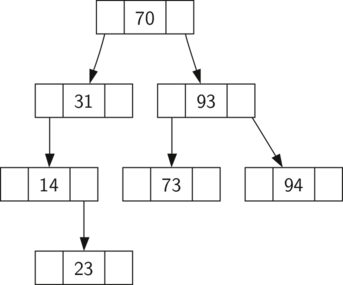
\includegraphics[height=0.8\textheight]{data_structures/graphics/bst.png}
    \end{center}
\end{frame}
\begin{frame}{Struktura danych - zbiór}
    \begin{itemize}
        \item set() \\
        \item zbiór danych w rozumieniu teorii zbiorów, czyli worek, do którego coś należy lub nie \\
        \item taki worek może być też wyobrażany jako słownik z tylko dwoma wartościami, True - gdy należy
        i False - gdy nie należy
    \end{itemize}
    Załóżmy że na kurs programowania chodzi 6 osób: \{Ala, Ela, Ola, Ula, Iza, Eberhard\}. \\
    Z rekurencją nie radzi sobie \{Ela, Ula\}. \\
    Metody HTTP są niezrozumiałe dla \{Ala, Ela, Iza\}. \\
    Algorytmów grafowych nie rozumieją \{Ela, Ola, Iza\}. \\
    Eberhard jako jedyny na zajęciach zadaje pytania, a w domu utrwala materiał - dlatego wszystko zrozumiał. \\
    Wymienione grupy osób są tematycznymi zbiorami, na których możemy wykonywać operację teoriomnogościowe:
    sumy, przecięcia, dopełnienia, itd.
\end{frame}

\begin{frame}{Ułamki}
    \begin{justify}
        Zauważmy, że:
        \begin{itemize}
            \item Każdy ułamek dziesiętny skończony lub nieskończony okresowy można zamienić w ułamek zwykły.
            Jedynie ułamka dziesiętnego nieskończonego nieokresowego nie da się zamienić. \\
            \item Każdy ułamek zwykły nieskracalny o mianowniku, będącym dzielnikiem
            jakiejś potęgi liczby 10 da się zamienić w ułamek dziesiętny skończony. \\
            \item Każdy ułamek zwykły nieskracalny o mianowniku niemającym tej własności
            jest równy pewnemu ułamkowi dziesiętnemu nieskończonemu okresowemu. \\
        \end{itemize}

        Ponieważ każdy ułamek zwykły to iloraz dwóch liczb całkowitych, więc każdy ułamek dziesiętny
        skończony lub nieskończony okresowy da się zapisać w postaci dwóch liczb całkowitych.
    \end{justify}
\end{frame}
\begin{frame}{Przeliczanie ułamków okresowych na zwykłe}
    \begin{gather*}
        0,(1234) = x | * 10000 \\
        1234,(1234) = 10000x \\
        1234,(1234) = 1234 + x \\
        1234 = 9999x \\
        x = \frac{1234}{9999} \\
        0,(1234) = \frac{1234}{9999} \\
    \end{gather*}
\end{frame}

\begin{frame}{Liczby rzeczywiste}
    Każda liczba rzeczywista jest jakimś ułamkiem dziesiętnym(również nieskończonym nieokresowym).

    Komputer jest maszyną skończoną i jako taki ma ograniczone zasoby. Z tego powodu w komputerze
    nie może przechowywać dokładnie niektórych rodzajów danych. Przykładem są liczby rzeczywiste,
    których jest nieskończenie wiele i których większość posiada nieskończone rozwinięcia dziesiętne.

    Rozpatrzmy liczbę $\pi$, która pozwoli nam lepiej zrozumieć problem.
    Poniżej przedstawiam jedynie pierwszych 1500 cyfr po przecinku jej rozwinięcia dziesiętnego.

\end{frame}
\begin{frame}{Pi, czyli 3,\dots}
    \centering
    14159265358979323846264338327950288419716939937510
    58209749445923078164062862089986280348253421170679
    82148086513282306647093844609550582231725359408128
    48111745028410270193852110555964462294895493038196
    44288109756659334461284756482337867831652712019091
    45648566923460348610454326648213393607260249141273
    72458700660631558817488152092096282925409171536436
    78925903600113305305488204665213841469519415116094
    33057270365759591953092186117381932611793105118548
    07446237996274956735188575272489122793818301194912
    98336733624406566430860213949463952247371907021798
    60943702770539217176293176752384674818467669405132
    00056812714526356082778577134275778960917363717872
    14684409012249534301465495853710507922796892589235
    42019956112129021960864034418159813629774771309960
\end{frame}
\begin{frame}{Pi, a dalej \dots}
    \centering
    51870721134999999837297804995105973173281609631859
    50244594553469083026425223082533446850352619311881
    71010003137838752886587533208381420617177669147303
    59825349042875546873115956286388235378759375195778
    18577805321712268066130019278766111959092164201989
    38095257201065485863278865936153381827968230301952
    03530185296899577362259941389124972177528347913151
    55748572424541506959508295331168617278558890750983
    81754637464939319255060400927701671139009848824012
    85836160356370766010471018194295559619894676783744
    94482553797747268471040475346462080466842590694912
    93313677028989152104752162056966024058038150193511
    25338243003558764024749647326391419927260426992279
    67823547816360093417216412199245863150302861829745
    55706749838505494588586926995690927210797509302955
\end{frame}
\begin{frame}{Liczby zmiennoprzecinkowe}
    Automat skończony jakim jest komputer nie mamy możliwości reprezentowania wszystkich liczb
    rzeczywistych, a jedynie ich mniej lub bardziej dokładne przybliżenia - mówi się, że float
    reprezentuje liczby zmiennoprzecinkowe, ponieważ w pamięci trzymane są w postaci znormalizowanej
    (czyli z przesuniętym przecinkiem) jako mantysa i wykładnik\footnote{zgodnie ze standardem IEEE 754}.
    \begin{center}
        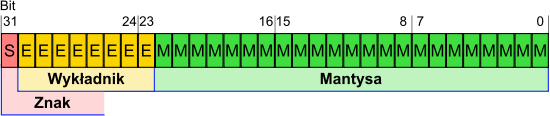
\includegraphics[width=0.7\textwidth]{data_structures/graphics/ieee_full.png}
    \end{center}
\end{frame}

\begin{frame}{Przeliczanie liczb zmiennoprzecinkowych}
    \begin{center}
        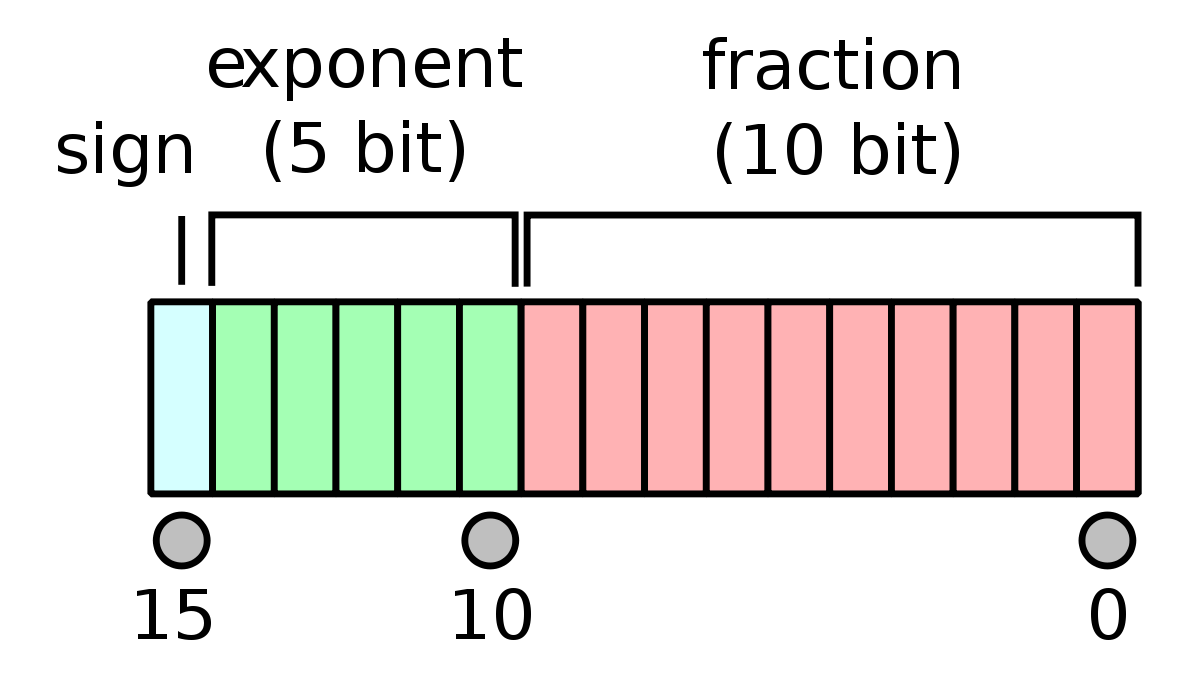
\includegraphics[height=0.2\textheight]{data_structures/graphics/ieee_half.png} \\
        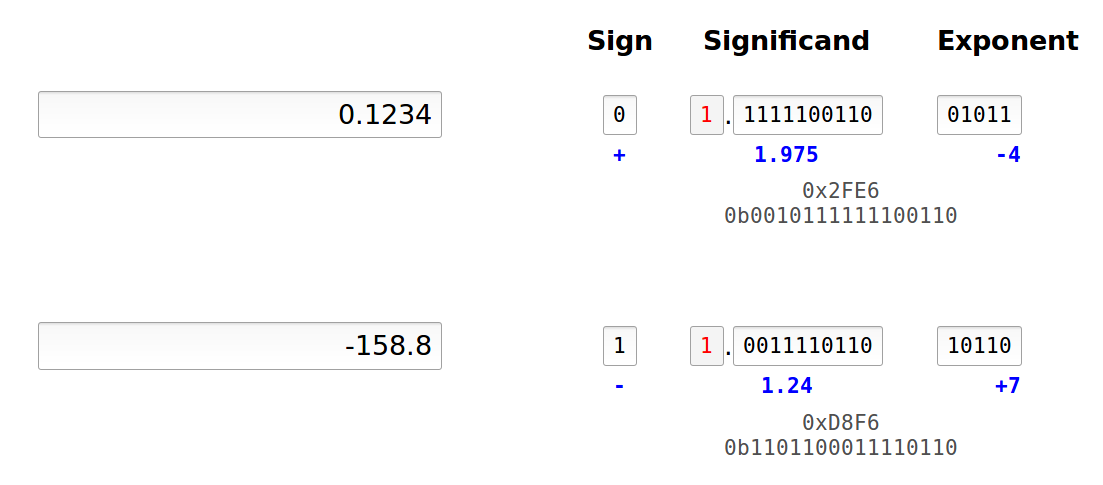
\includegraphics[height=0.45\textheight]{data_structures/graphics/calculations.png}
    \end{center}
    Program do przeliczania dla różnych precyzji: \url{http://weitz.de/ieee/}
\end{frame}

\section{Płaski model pamięci}\label{sec:memory}
\begin{frame}
    \begin{table}
        \centering
        \begin{tabular}{rc|c|}
            \cline{3-3}
            & & \\
            \cline{3-3}
            0x7999 & \longrightarrow & \cdots \\
            \cline{3-3}
            0x8000 & \longrightarrow & 00101100 \\
            \cline{3-3}
            0x8001 & \longrightarrow & 01110010 \\
            \cline{3-3}
            0x8002 & \longrightarrow & 10010101 \\
            \cline{3-3}
            0x8003 & \longrightarrow & 11011011 \\
            \cline{3-3}
            0x8004 & \longrightarrow & 10111011 \\
            \cline{3-3}
            0x8005 & \longrightarrow & 11110010 \\
            \cline{3-3}
            0x8006 & \longrightarrow & 01110001 \\
            \cline{3-3}
            0x8007 & \longrightarrow & 10110011 \\
            \cline{3-3}
            0x8008 & \longrightarrow & \cdots \\
            \cline{3-3}
            & & \\
            \cline{3-3}
        \end{tabular}
    \end{table}
\end{frame}